\section{Part 5}
\subsection*{Mixture Models}
\[\Pr(x\mid \pi, \Theta)=\sum_{c=1}^k \pi_c \Pr(x\mid \Theta_c)\]
Latent-variable representation of mixtures with cluster variables $z^i$\\
Ancestral sampling \\
Responsibility = prob example belongs to cluster\\
\subsection*{Mixture of Gaussians}
Prob as convex comb. of Gaussian densities\\
\[\Pr(x\mid \pi, \mu,\Sigma)=\sum_{c=1}^k \pi_c \Pr(x\mid \mu_c,\Sigma_c)\]
Model arbitrary continuous indentities ("universal approximator")\\
\subsection*{Mixture of Bernoullis}
Mixture of Bernoullis model dependencies btw discrete variables\\
\[\Pr(x\mid \pi, \Theta)=\sum_{c=1}^k \pi_c \prod\theta_{cj}\]
Soft-clustering of examples
\subsection*{Notation}
\begin{enumerate}
    \item \[\pi\in{[0,1]}^k, \sum_i\pi_i=1\]
    $\pi_c$ is prior prob that example is in cluster $c$. \\
    Parameter learned from data.
    \item \[R\in{[0,1]}^{n\times k},\sum_c r_c^i=1\]
    Responsibility $r_c^i$ is posterior prob that example $i$ is in cluster $c$.\\
    Computing values is inference task (assumes known params)
    \item \[z\in\{1,2,\dots,k\}^n\]
    Category $z^i$ is actual mixture generating example $i$.\\
    Nuissance parameter - unknown variable not a parameter
\end{enumerate}
\subsection*{Imputation}
Alternate btw finding best value of latent variables, and updating params
\begin{enumerate}
    \item Find most likely cluster $z^i$ for each example $i$
    \[z^i\in\argmax_c\Pr(z^i=c\mid x^i,\Theta)\]
    \item Update mixture probs as proportion of examples cluster is responsible for
    \[\pi_c=\frac{1}{n}\sum_{i=1}^n I[z^i=c]\]
    \item Update prod of Bernoullis based on examples cluster is responsible for
    \[\theta_{cj}=\frac{1}{n_c}\sum_{i=1}^n I[z^i=c] x_j^i\]
\end{enumerate}
\subsection*{Expectation Maximization (EM)}
EM : Algorithm for optimization w hidden variables\\
Instead of imputation, "soft" assignments to hidden variables\\
Maximizes log likelihood, weighted by imputations of hidden variables\\
Local optimum\\
General algorithm for parameter learning with missing data
\subsection*{EM for Prod of Bernoullis}
\begin{enumerate}
    \item Find responsibility of cluster $z^i$ for each example $i$
    \[r_c^i=\Pr(z^i=c\mid x^i,\Theta)\]
    \item Update mixture probs as proportion of examples cluster is responsible for
    \[\pi_c=\frac{1}{n}\sum_{i=1}^n r_c^i\]
    \item Update prod of Bernoullis based on examples cluster is responsible for
    \[\theta_{cj}=\frac{1}{\sum_{i=1}^n r_c^i}\sum_{i=1}^n r_c^i x_j^i\]
\end{enumerate}
\subsection*{General EM}
\begin{enumerate}
    \item E-Step: Compute responsibilities $r_c^i,\forall i,c$ for current $\Theta^t$.
    \item M-Step: Optimize weighted complete-data log-likelihood
    \[\Theta^{t+1}\in\argmax_{\Theta}\sum_{i=1}^n\sum_{z^i=1}^k r_c^i \log\Pr(x^i,z^i\mid\Theta)\]
\end{enumerate}
\subsection*{EM Properties}
\begin{enumerate}
    \item Useful when complete-data log-likelihood easy to optimize
    \item Monotonically increases likelihood $\Pr(X\mid \Theta^{t+1})\geq\Pr(X\mid\Theta^t)$
    \item Does not need step size
    \item Tends to satisfy constraints automatically
    \item Iterations are parameterization independent
    \item Notorious for converging to bad local optima (to be expected for hard problems)
    \item Converges to stationary point under weak assumptions
    \item At least as fast as gradient descent with constant step size
    \item Converges faster as entropy of hidden variables decreases
    \item Arbitrarily faster than gradient descent in "best case"
\end{enumerate}
\subsection*{Kernel Density Estimation (KDE)}
KDE : Non-parametric density method\\
\[\Pr(x^i)=\frac{1}{n}\sum_{j=1}^n\Pr(x^i\mid x^j,\sigma^2 I)\]
Center a mixture on each datapoint\\
Data visualization and low-dimensional density estimation\\
Basis of mean-shift clustering
\subsection*{Hidden Markov Models (HMMs)}
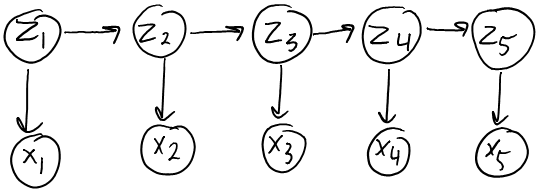
\includegraphics[scale=.6]{contents/hmm.png}
\[\Pr(x_1,\dots,x_d,z_1,\dots,z_d)
=\Pr(z_1)\prod_{j=2}^d\Pr(z_j\mid z_{j-1})\prod_{j=1}^d\Pr(x_j\mid z_j)\]
HMMs model time-series with hidden per-time cluster\\
\subsection*{Restricted Boltzmann Machines (RBMs)}
RBMs : UGMs with binary hidden variables\\
\[\Pr(x,z)=\frac{1}{Z}\prod_{j=1}^d\phi_j(x_j)
\prod_{c=1}^k\phi_c(z_c)\prod_{j=1}^d\prod_{c=1}^k\phi_{jc}(x_j,z_c)\]
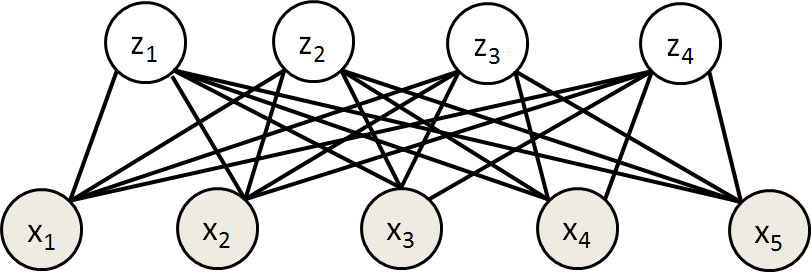
\includegraphics[width=\linewidth]{contents/rbm.png}
Normally with log-linear parameterization
\[\Pr(x,z)\propto \exp\left(
    \sum_{j=1}^d w_j x_j + \sum_{c=1}^k v_c z_c 
    + \sum_{j=1}^d\sum_{c=1}^k w_{jc}x_j z_c\right)\]
Pairwise edges only btw visible and hidden\\
    Efficient block Gibbs sampling for inference/learning\\
Deep Boltzmann machines stack RBMs into deep density estimation model